\documentclass[a4paper,12pt]{ujarticle}
\usepackage{listings,jlisting}
\usepackage[top=15truemm,bottom=15truemm,left=20truemm,right=20truemm]{geometry}
\usepackage[dvips]{graphicx}
\usepackage{siunitx}
\usepackage{multirow}
\usepackage{makecell}
\begin{document}
\title{マイクロコンピュータ 後期期末レポート}
\author{電気情報工学科2年 \\ E1533 西総一朗}
\date{2017年2月10日提出}
\maketitle
\begin{itemize}
 \item \large 光が流れるプログラム(片道バージョン)
 \item 光が流れるプログラム(往復バージョン)
 \item パルスモータ1-2相励磁プログラム
 \item 電子サイコロのプログラム
 \item タイマ割り込み制御プログラム
\end{itemize}
\clearpage
\tableofcontents
\clearpage
 \section{リスト5-5(光が流れるプログラム(片道バージョン))}
  \subsection{プログラム説明}
  8個あるLEDの内1個を左端から右へ0.5秒間隔で順次点灯することによって、光が流れるように見えるプログラム。
  \subsection{フローチャート}
  このプログラムのフローチャートを図\ref{fig:flow_5-5}に示す。
  \begin{figure}[htbp]
   \begin{center}
    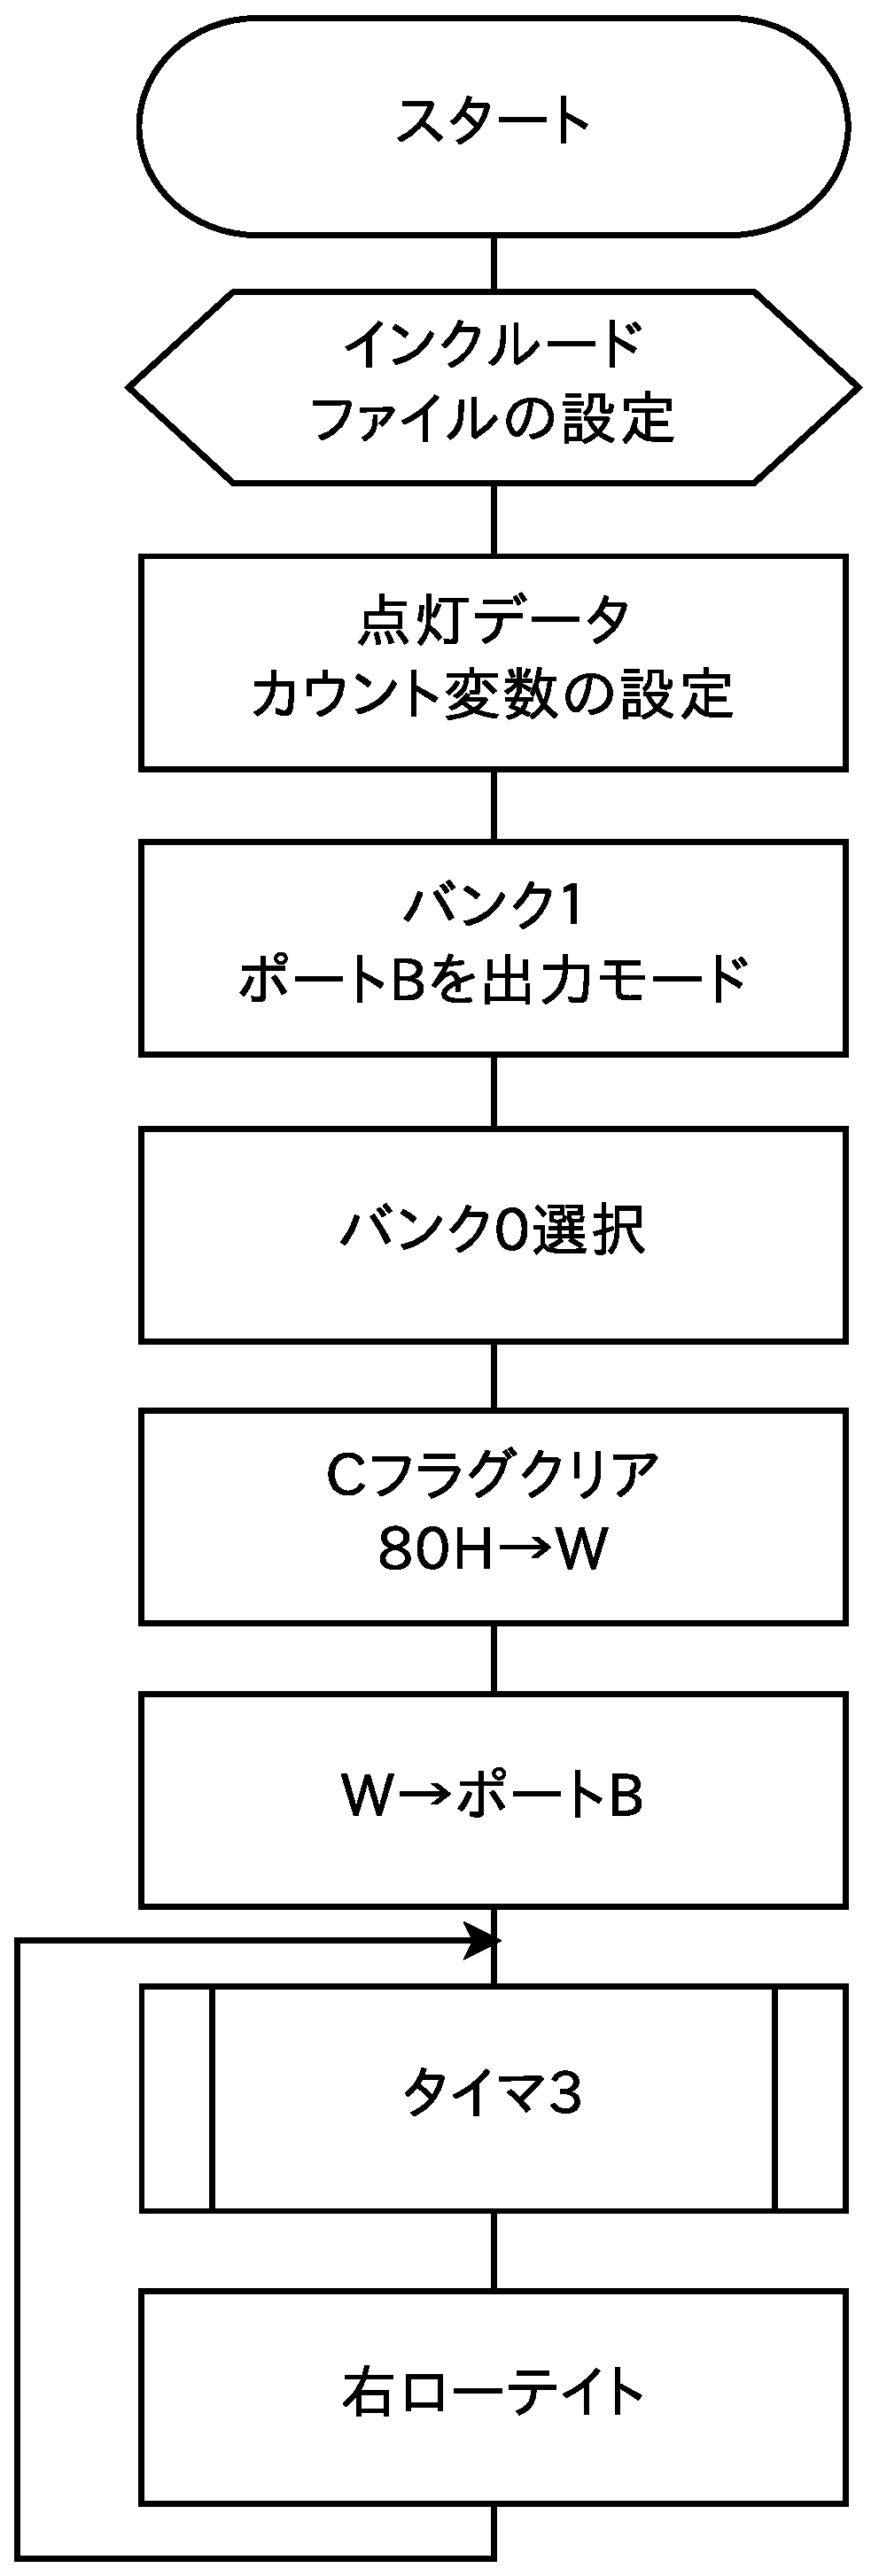
\includegraphics[height=185mm]{Diagram5-5.eps}
   \end{center}
   \caption{光が流れるプログラム ( 片道バージョン )のフローチャート}
   \label{fig:flow_5-5}
  \end{figure}
   \clearpage
  \subsection{ソースコード}
   \begin{lstinputlisting}[basicstyle=\ttfamily\footnotesize, frame=single,numbers=left]
    {../5-5/5-5.asm}
   \end{lstinputlisting}
   \clearpage
  \subsection{実行結果・考察}
   \begin{figure}[htbp]
    \begin{center}
     \begin{tabular}{c|cc}\hline
      状態&76543210 & C \\ \hline
      \multirow{2}{*}{1}&{80}$_{16}$ = 10000000$_2$ \\
      &●○○○○○○○ & □\\ \hline
      \multirow{2}{*}{2}&{40}$_{16}$ = 01000000$_2$ \\
      &○●○○○○○○ & □\\ \hline
      \multirow{2}{*}{3}&{20}$_{16}$ = 00100000$_2$ \\
      &○○●○○○○○ & □\\ \hline
      \multirow{2}{*}{4}&{10}$_{16}$ = 00010000$_2$ \\
      &○○○●○○○○ & □\\ \hline
      \multirow{2}{*}{5}&{08}$_{16}$  = 00001000$_2$ \\
      &○○○○●○○○ & □\\ \hline
      \multirow{2}{*}{6}&{04}$_{16}$  = 00000100$_2$ \\
      &○○○○○●○○ & □\\ \hline
      \multirow{2}{*}{7}&{02}$_{16}$  = 00000010$_2$ \\
      &○○○○○○●○ & □\\ \hline
      \multirow{2}{*}{8}&{01}$_{16}$  = 00000001$_2$ \\
      &○○○○○○○● & □\\ \hline
      \multirow{2}{*}{9}&{00}$_{16}$  = 00000000$_2$ \\
      &○○○○○○○○ & ■\\ \hline
     \end{tabular}\\
     ●:LED点灯 ○:LED消灯,■:Cフラグ1 □:Cフラグ0
    \end{center}
    \caption{光が流れるプログラム ( 片道バージョン )の実行結果。上の数字はポートBの値を表す。}
    \label{fig:out_5-5}
   \end{figure}
   図\ref{fig:out_5-5}はポートBの出力状態を表している。0.5秒毎にLEDの点灯箇所が右に移動していき(状態1〜9)、右端に到達する(状態9)と全てのLEDが消灯する。この一連の動作を繰り返す。ローテイト(RRF)命令はCフラグを経由してデータを1ビット右にシフトするのでCフラグにデータが存在するときには全てのLEDが消灯している。\\

   このプログラムのタイマについて考えてみる。
   PICのクロック周波数は$10\si{\mega\hertz}$なので、1クロックは
    \[
     \frac{1}{10\si{\mega\hertz}} = \SI{0.1}{\mu\second}
    \]
    4クロックで1サイクルなので、1サイクルは
    \[
     \SI{0.1}{\mu\second} \times 4 = \SI{0.4}{\mu\second}
    \]
     \begin{figure}[h]
      \begin{center}
       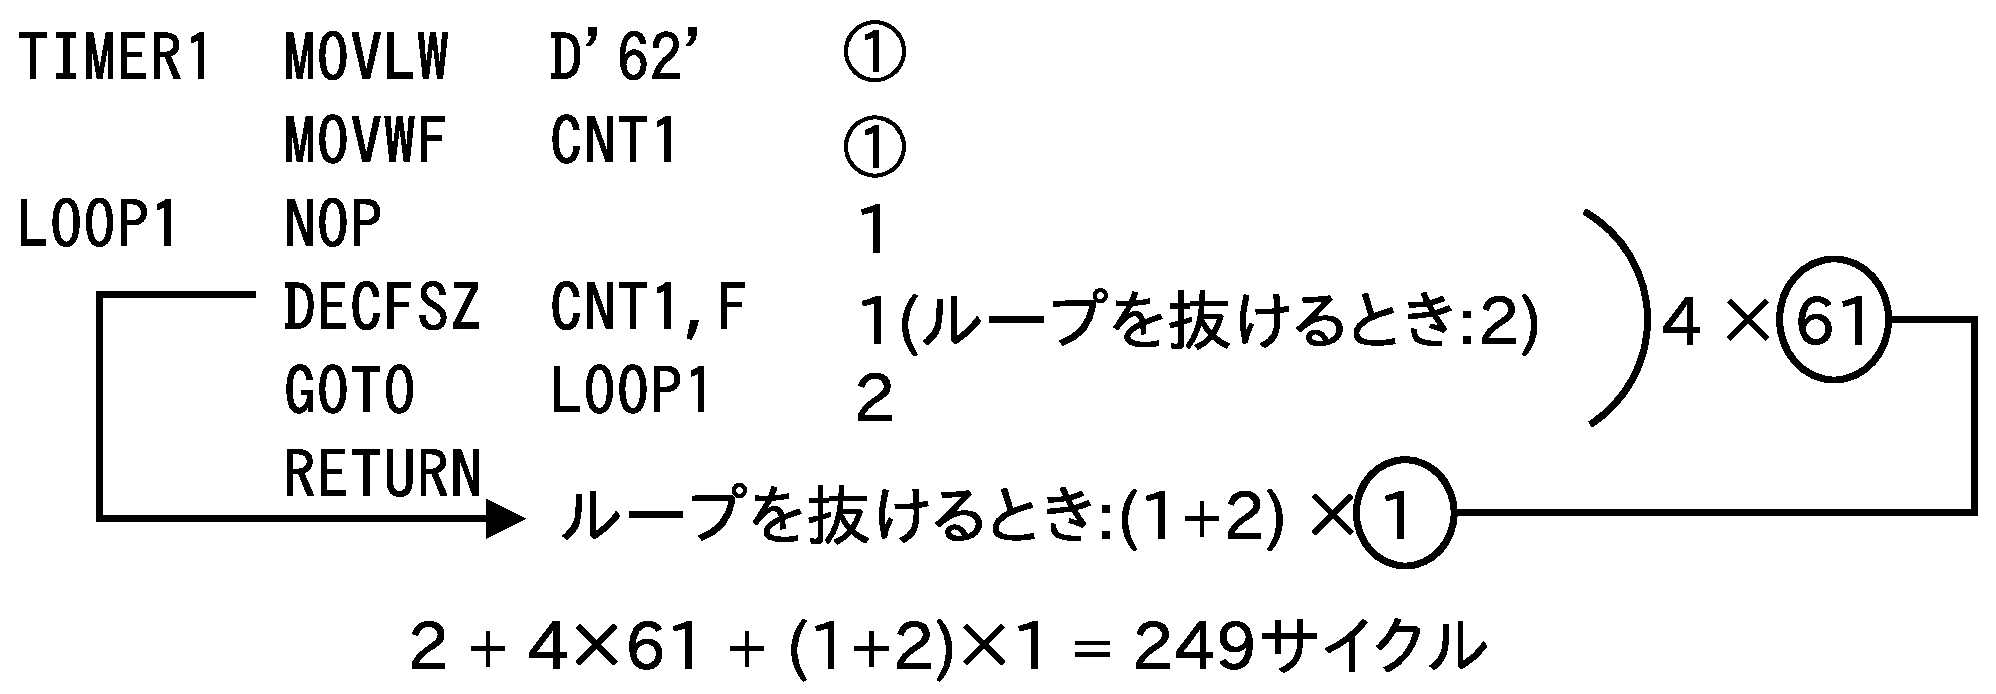
\includegraphics[width=130mm]{Diagram5.eps}
      \end{center}
      \caption{サイクル数の考え方}
      \label{fig:sicle}
     \end{figure}
     TIMER1のサイクル数は図\ref{fig:sicle}より、249サイクルだとわかり、
     \[
      \SI{0.4}{\mu\second} \times 249 = \SI{99.6}{\mu\second} \approx \SI{0.1}{\milli\second}
     \]
     TIMER1では$\SI{0.1}{\milli\second}$かかる。\\
     このTIMER1をTIMER2では100回呼び出し、TIMER3はTIMER2を50回呼び出しているので、
     \[
      \SI{0.1}{\milli\second} \times 100 \times 50 = \SI{50}{\milli\second} = \SI{0.5}{\second}
     \]
     よってTIMER1,TIMER2,TIMER3の合計で$\SI{0.5}{\second}$のタイマールーチンであることがわかる。\\

     次に光の移動方向について考えてみる。
     このプログラムにおいて、光の移動方向を決めているのは
      \begin{lstlisting}[basicstyle=\ttfamily\footnotesize, frame=single]
 9行目     LEDD    EQU     80H     ;LEDの点灯データの設定

24行目     RRF     PORTB,1         ;ポートBを1ビット右にローテイト
      \end{lstlisting}
      この2つなので次のように変更すれば左方向に移動するようになる。
      \begin{lstlisting}[basicstyle=\ttfamily\footnotesize, frame=single]
 9行目     LEDD    EQU     01H     ;LEDの点灯データの設定

24行目     RLF     PORTB,1         ;ポートBを1ビット右にローテイト
      \end{lstlisting}
      RLF命令もRRF命令と同様に、C フラグを経由してデータを 1 ビット左にシフトするので C フラグにデータが存在するときには全ての LED が消灯している。

      LEDの移動時間$S$を調整するにはTIMER1の0.1ミリ秒を基準にして、
      \begin{eqnarray*}
       S = \SI{0.1}{\milli\second} \times {\rm TIMER2 \times TIMER3} \\
       {\rm TIMER2 \le 255},\ {\rm TIMER3 \le 255}
      \end{eqnarray*}
      TIMER2とTIMER3とで移動時間$S$を調整する。
      \clearpage
 \section{リスト5-6(光が流れるプログラム(往復バージョン))}
  \subsection{プログラム説明}
  8個あるLEDの内1個を左端から右へ0.5秒間隔で順次点灯していき、右端に到達すると移動方向を逆にして左端に向かう。光が左から右へ流れるように見え、右端に到達すると右から左へ流れるように見えるプログラム。
  \subsection{フローチャート}
  このプログラムのフローチャートを図\ref{fig:flow_5-6}に示す。
  \begin{figure}[htbp]
   \begin{center}
    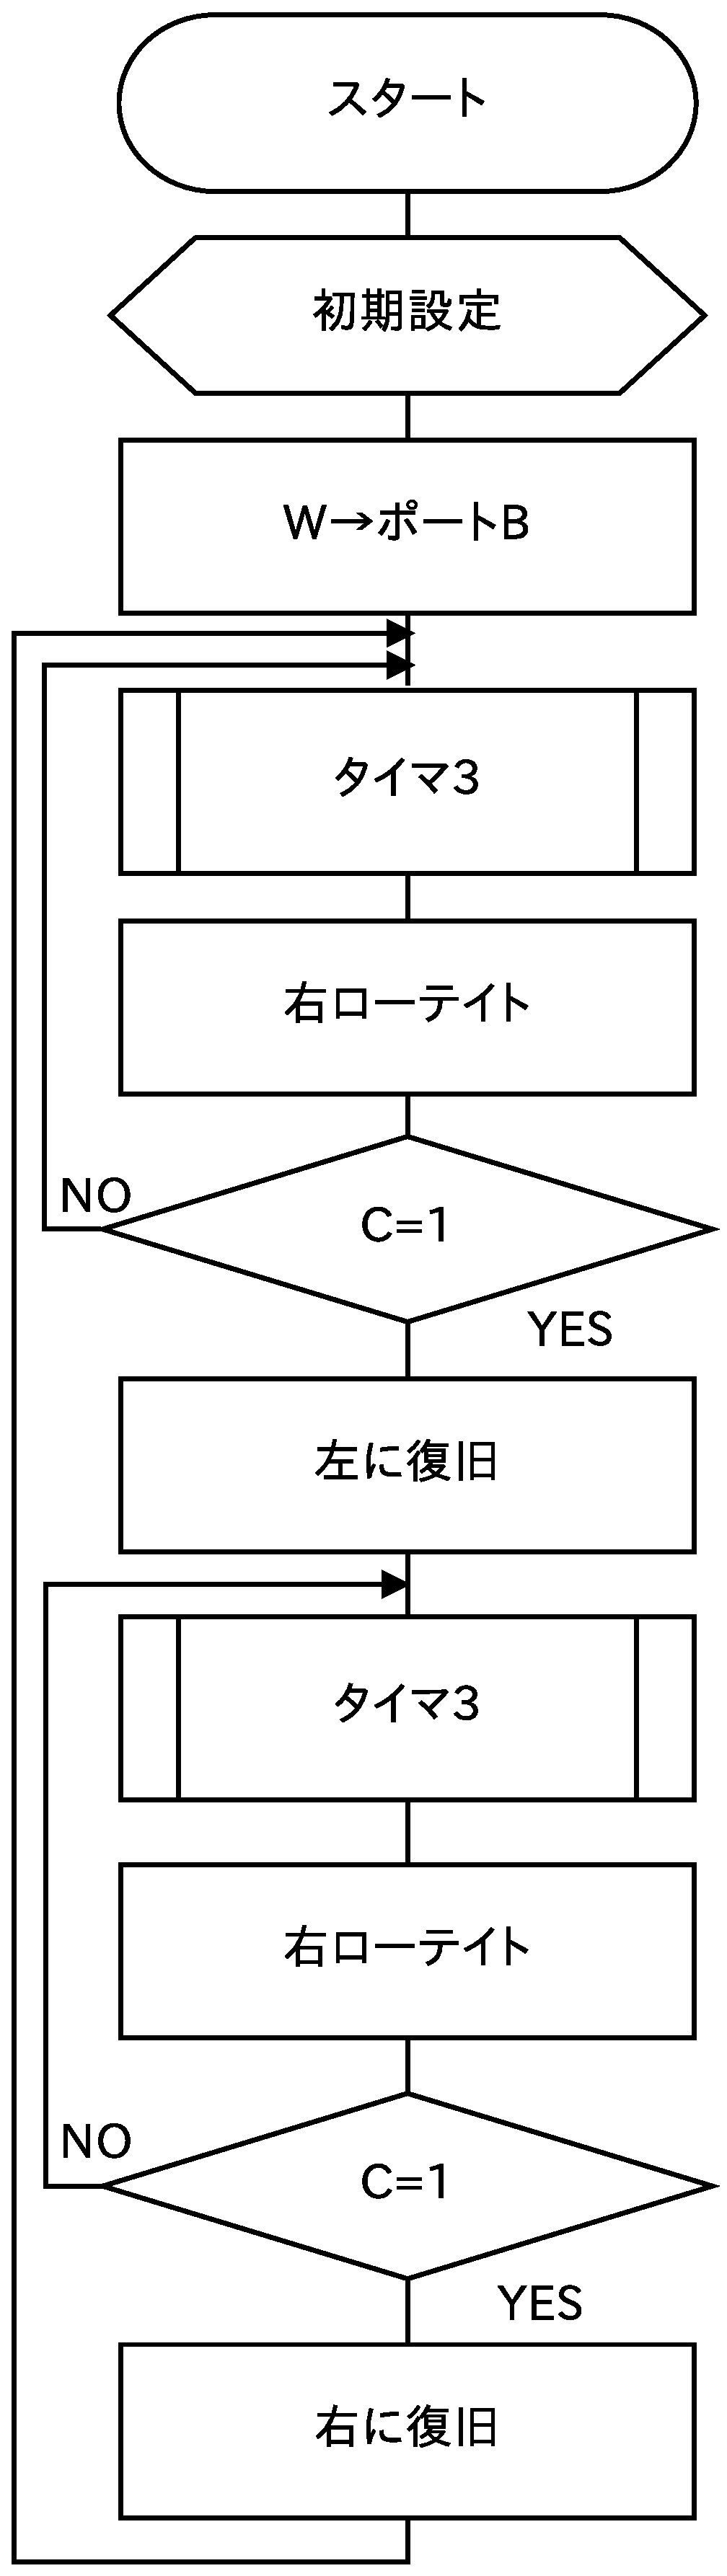
\includegraphics[height=180mm]{Diagram5-6.eps}
   \end{center}
   \caption{光が流れるプログラム ( 往復バージョン )のフローチャート}
   \label{fig:flow_5-6}
  \end{figure}
  \clearpage
  \subsection{ソースコード}
   \begin{lstinputlisting}[basicstyle=\ttfamily\footnotesize, frame=single,numbers=left]
    {../5-6/5-6.asm}
   \end{lstinputlisting}
  \subsection{実行結果・考察}
  \begin{figure}[htbp]
   \begin{center}
    \begin{tabular}{c|c||c|c}\hline
     状態&76543210       &状態 &76543210 \\ \hline
     \multirow{2}{*}{1}&{80}$_{16}$ = 10000000$_2$& \multirow{2}{*}{8}&{01}$_{16}$  = 00000001$_2$ \\
     &●○○○○○○○            & &○○○○○○○● \\ \hline
     \multirow{2}{*}{2}&{40}$_{16}$ = 01000000$_2$ & \multirow{2}{*}{9}&{02}$_{16}$  = 00000010$_2$ \\
     &○●○○○○○○            & &○○○○○○●○ \\ \hline
     \multirow{2}{*}{3}&{20}$_{16}$ = 00100000$_2$ & \multirow{2}{*}{10}&{04}$_{16}$  = 00000100$_2$ \\
     &○○●○○○○○            & &○○○○○●○○ \\ \hline
     \multirow{2}{*}{4}&{10}$_{16}$ = 00010000$_2$ & \multirow{2}{*}{11}&{08}$_{16}$  = 00001000$_2$ \\
     &○○○●○○○○            & &○○○○●○○○ \\ \hline
     \multirow{2}{*}{5}&{08}$_{16}$  = 00001000$_2$ &\multirow{2}{*}{12}& {10}$_{16}$ = 00010000$_2$ \\
     &○○○○●○○○            & &○○○●○○○○ \\ \hline
     \multirow{2}{*}{6}&{04}$_{16}$  = 00000100$_2$ &\multirow{2}{*}{13}& {20}$_{16}$ = 00100000$_2$ \\
     &○○○○○●○○            & &○○●○○○○○ \\ \hline
     \multirow{2}{*}{7}&{02}$_{16}$  = 00000010$_2$ &\multirow{2}{*}{14}&{40}$_{16}$ = 01000000$_2$ \\
     &○○○○○○●○            & &○●○○○○○○ \\ \hline
    \end{tabular}\\
     ●:LED点灯 ○:LED消灯
     \caption{光が流れるプログラム ( 往復バージョン )の実行結果。上の数字はポートBの値を表す。}
     \label{fig:out_5-6}
   \end{center}
  \end{figure}
   図\ref{fig:out_5-6}はポートBの出力状態を表している。
   0.2秒毎にLEDの点灯箇所が右に移動していき(状態1〜7)右端(状態8)に到達したら、移動方向を左に反転する(状態8〜14)。
   左端(状態1)に到達したら再びこの一連の動作を繰り返す。
   ローテイト(RRF,RLF)命令はCフラグを経由してデータを1ビット(右,左)にシフトするのでCフラグにデータが存在するかどうかで、
   光が右端(0ビット目)または左端(7ビット目)に移動したことを判定している。
   Cフラグが1の場合はオーバーフローかアンダーフローしているので、
   図\ref{fig:under}に過分ローテートの復旧を示す。状態9の次に状態Uがくるが、
   状態Uに到達したらすぐに過分ローテートの復旧するためにRLF命令を2回実行することで、状態10に移行し光がなめらかに移動するように見える。

   \begin{figure}[htbp]
    \begin{center}
      \begin{tabular}{c|cc|l}\hline
      状態&76543210 & C  &\makecell[c]{説明} \\ \hline
      \multirow{2}{*}{9}&{01}$_{16}$ = 00000001$_2$ && \multirow{2}{*}{0ビット目点灯} \\
      &○○○○○○○● & □ & \\ \hline
      \multirow{2}{*}{U}&{00}$_{16}$ = 00000000$_2$ && \multirow{2}{*}{Cフラグにアンダーフロー} \\
      &○○○○○○○○ & ■ & \\ \hline
      \multirow{2}{*}{10}&{02}$_{16}$ = 00000010$_2$&& \multirow{2}{*}{過分ローテート復旧(RLF $\times$ 2)} \\
      &○○○○○○●○ & □ & \\ \hline
      \end{tabular}\\
     ●:LED点灯 ○:LED消灯,■:Cフラグ1 □:Cフラグ0
     \caption{過分ローテート復旧の例。上の数字はポートBの値を表す。}
     \label{fig:under}
    \end{center}
   \end{figure}
   光の移動方向については、Cフラグでの判定と過分ローテートの復旧を行っているため、LEDの点灯データを変えるだけで、移動方向を変えられる。プログラムの9行目
   \begin{lstlisting}[basicstyle=\ttfamily\footnotesize, frame=single]
9行目    LEDD     EQU     80H    ;左端から右方向にスタート
   \end{lstlisting}
   を次のように変更すれば、スタート時の移動方向を反対にできる。
   \begin{lstlisting}[basicstyle=\ttfamily\footnotesize, frame=single]
9行目    LEDD     EQU     01H    ;右端から左方向にスタート
   \end{lstlisting}

   \vspace{3mm}

   次に過分ローテイトの復旧がない場合について考えてみる。
    \begin{figure}[htbp]
     \begin{center}
      \begin{tabular}{c|cc|l}\hline
       状態&76543210 & C  &\makecell[c]{説明}\\ \hline
       \multirow{2}{*}{7}&{02}$_{16}$ = 00000010$_2$ && \multirow{2}{*}{1ビット目点灯} \\
       &○○○○○○●○ & □ & \\ \hline
       \multirow{2}{*}{8}&{01}$_{16}$ = 00000001$_2$ && \multirow{2}{*}{0ビット目点灯} \\
       &○○○○○○○● & □ & \\ \hline
       \multirow{2}{*}{U}&{00}$_{16}$ = 00000000$_2$ && \multirow{2}{*}{Cフラグにアンダーフロー} \\
       &○○○○○○○○ & ■ & \\ \hline
       \multirow{2}{*}{8}&{01}$_{16}$ = 00000001$_2$ && \multirow{2}{*}{0ビット目点灯} \\
       &○○○○○○○● & □ & \\ \hline
       \multirow{2}{*}{9}&{02}$_{16}$ = 00000010$_2$ && \multirow{2}{*}{1ビット目点灯} \\
       &○○○○○○●○ & □ & \\ \hline
      \end{tabular}\\
      ●:LED点灯 ○:LED消灯,■:Cフラグ1 □:Cフラグ0
      \caption{過分ローテート復旧がない場合。上の数字はポートBの値を表す。}
      \label{fig:under_less}
     \end{center}
    \end{figure}

    図\ref{fig:under_less}のように過分ローテイトの復旧がないと、全てのLEDが0.5秒間点灯しないので不自然に移動してるように見える。
    \clearpage
 \section{リスト 5-12(パルスモータ 1-2 相励磁プログラム)}
  \subsection{プログラム説明}
    1相励磁と2相励磁を交互に繰り返して、パルスモータを制御するプログラム。
    時計回りに配置されている4つのコイル$X$,$Y$,$\bar{X}$,$\bar{Y}$について順に電流を流していく。
    4つのコイル$X$,$Y$,$\bar{X}$,$\bar{Y}$はこの順に$90^\circ$ずつ配置されている。
    励磁の順序は最初に$X$、次に$X$と$Y$、次に$Y$のように行う。
    すなわち、コイルを1つ励磁し、次に隣のコイルと合わせて2つ励磁し、次に隣のコイル1つだけを励磁するのを繰り返す。
    この動作をまとめると表\ref{table:1-2}になる。表\ref{table:1-2}の$X$,$Y$,$\bar{X}$,$\bar{Y}$の組をデータとして予めファイルレジスタに入れておいて、これらを順に呼び出して出力する。
    \begin{table}[h]
     \begin{center}
      \caption{1-2相励磁の場合のコイルに流す電流の組の順序}
      \label{table:1-2}
      \vspace{2mm}
      \begin{tabular}[h]{|c||c|c|c|c|c|c|c|c|}\hline
       &1&2&3&4&5&6&7&8 \\ \hline \hline
       $X$&1&1&0&0&0&0&0&1 \\
       $Y$&0&1&1&1&0&0&0&0 \\
       $\bar{X}$&0&0&0&1&1&1&0&0 \\
       $\bar{Y}$&0&0&0&0&0&1&1&1 \\ \hline \hline
      データ &$8_{16}$&$C_{16}$&$4_{16}$&$6_{16}$&$2_{16}$&$3_{16}$&$1_{16}$&$9_{16}$ \\ \hline
      \end{tabular}
     \end{center}
    \end{table}
  \subsection{フローチャート}
    図\ref{fig:flow_5-12}にこのプログラムのフローチャートを示す。
  \subsection{ソースコード}
    \begin{lstinputlisting}[basicstyle=\ttfamily\footnotesize, frame=single,numbers=left]
     {../5-12/5-12.asm}
    \end{lstinputlisting}

    \begin{figure}[htbp]
     \begin{center}
      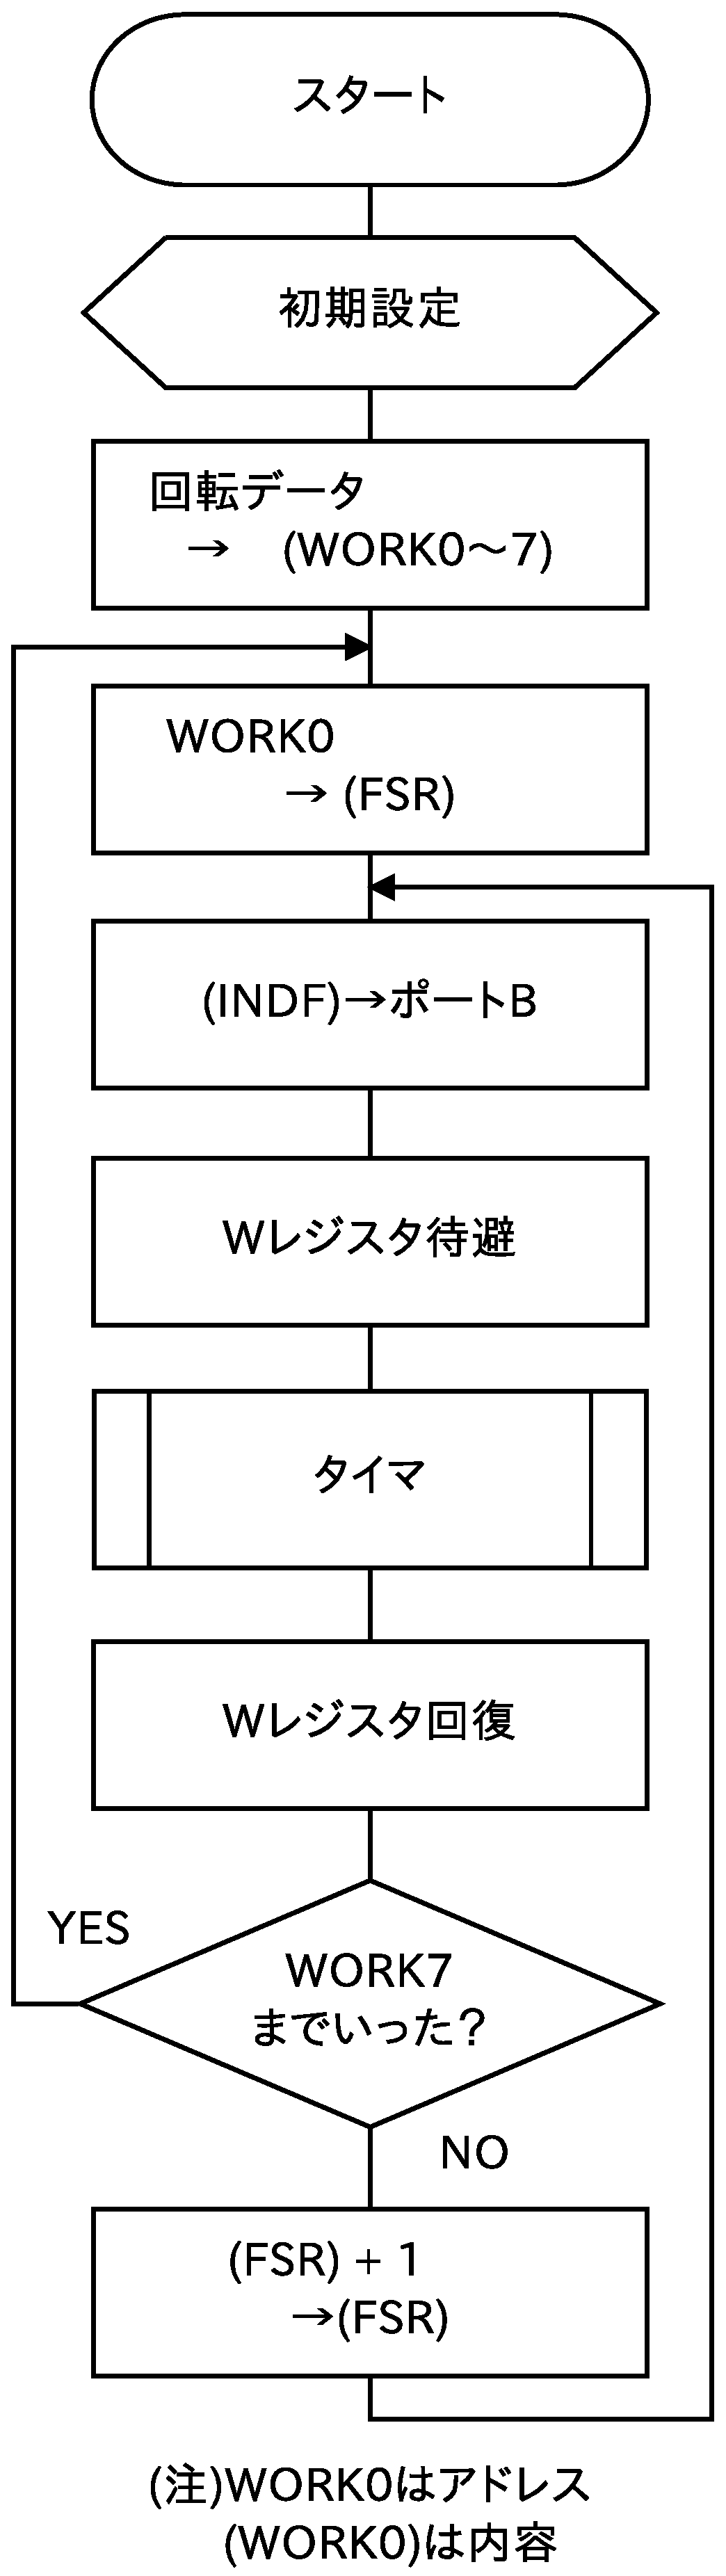
\includegraphics[height=230mm]{Diagram5-12.eps}
     \end{center}
     \caption{パルスモータ 1-2 相励磁プログラムのフローチャート}
     \label{fig:flow_5-12}
    \end{figure}
    \subsection{実行結果・考察}
    実行する前にボードのRB0をDOWNにスイッチしておく。実験で使用したボードにはパルスモータが接続されていないのでLEDで動作を確認する。
    \begin{figure}[htbp]
     \begin{center}
       \begin{tabular}{c|c|c}\hline
        \multirow{2}{*}{状態}&76543210 & \multirow{2}{*}{データ}\\
        &    $X$\,$Y$\,$\bar{X}$\,$\bar{Y}$\\ \hline
         1&○○○○●○○○ & $8_{16}=00001000_2$ \\
         2&○○○○●●○○ & C$_{16}=00001100_2$\\
         3&○○○○○●○○ & $4_{16}=00000100_2$\\
         4&○○○○○●●○ & $6_{16}=00000110_2$\\
         5&○○○○○○●○ & $2_{16}=00000010_2$\\
         6&○○○○○○●● & $3_{16}=00000011_2$\\
         7&○○○○○○○● & $1_{16}=00000001_2$\\
         8&○○○○●○○● & $9_{16}=00001001_2$\\ \hline
       \end{tabular}\\
      ●:LED点灯 ○:LED消灯
      \caption{パルスモータ 1-2 相励磁プログラムの実行結果}
      \label{fig:out_5-12}
     \end{center}
    \end{figure}

    図\ref{fig:out_5-12}はポートBの出力状態を表している。8個のLEDの内右側の4つが
    それぞれコイル$X$,$Y$,$\bar{X}$,$\bar{Y}$に対応している。
    状態1〜8はLEDの点灯状態で、0.5秒毎に移行していく。状態8の次は状態1に戻る。
    各コイルでみると対応するLEDが1.5秒点灯して、2.5秒消灯するように変化している。
    各コイルの動作は1秒ずれているので、1相励磁と2相励磁が交互に繰り返す様子が確認できた。

    この動作を実現するためにあらかじめデータをメモリに入れておいて、それを読みだしてPORTBにセットしている。
    FSRレジスタの内容を1ずつ変えて、INDFレジスタを読みだすと
    FSRレジスタの内容が指すメモリアドレスにアクセスすることで読み出しを実現している。
    つまり間接アドレッシング方式を用いている。

    読みだす順序を変えるだけで、モーターを反転させることができる。
    そのためには読みだす最初のアドレスを反対からにして読みだすアドレスを1つずつ減らしていく。
     \begin{lstlisting}[basicstyle=\ttfamily\footnotesize, frame=single]
47行目      NEW  MOVLW  WORK0
54行目           SUBWF  WORK7
58行目           INCF   FSR,F
     \end{lstlisting}
     このコードを
     \begin{lstlisting}[basicstyle=\ttfamily\footnotesize, frame=single]
47行目      NEW  MOVLW  WORK7
54行目           SUBWF  WORK0
58行目           DECF   FSR,F
     \end{lstlisting}
     このように変えるとよい。

     回転の速さはTIMER3のカウント数で調整すればよい。
     \\

     1相制御にするにはWORK0〜WORK7に格納するデータを
     \begin{table}[htbp]
      \begin{center}
       \caption{1相励磁のデータ}
       \label{table:1-data}
       \begin{tabular}{|c|c|}
        \hline
        WORK0 & 08$_{16}=00001000_2$\\
        WORK1 & 04$_{16}=00000100_2$\\
        WORK2 & 02$_{16}=00000010_2$\\
        WORK3 & 01$_{16}=00000001_2$\\ \hline
       \end{tabular}
      \end{center}
     \end{table}
     表\ref{table:1-data}のようにして、WORK5〜WORK7は使わず、コードの54行目を
     \begin{lstlisting}[basicstyle=\ttfamily\footnotesize, frame=single]
54行目           SUBWF  WORK3
     \end{lstlisting}
     のように変えれば良い。
     \\

     2相制御なら、同様に表\ref{table:2-data}のデータを与えればよい。
     \begin{table}[htbp]
      \begin{center}
       \caption{2相励磁のデータ}
       \label{table:2-data}
       \begin{tabular}{|c|c|} \hline
        WORK0 & 0C$_{16}=00001100_2$\\
        WORK1 & 06$_{16}=00000110_2$\\
        WORK2 & 03$_{16}=00000011_2$\\
        WORK3 & 09$_{16}=00001001_2$\\ \hline
       \end{tabular}
      \end{center}
     \end{table}

     このようにテーブルを与えて順に読みだす方式は非常に汎用的な制御方法と考えられる。
     \clearpage
\section{電子サイコロのプログラム}
  \subsection{プログラム説明}
  メインルーチンではINTピンによる割り込みを許可する。割り込みの立ち上がりのエッヂで割り込みが
  入るように設定する。ボタン(RB0)のみ入力に設定し、RB1〜RB7はLEDの出力に設定する。
  ポートBをクリアしてLEDを消灯させる。
  ボタン(RBO)を押されるまで、Wレジスタに1番目から6番目までの点灯データを書き込む。
  ボタン(RB0)が押されると割り込みが発生して、割り込みルーチンないでWレジスタの書き込みを
  禁止して、Wレジスタの内容をポートBに出力しLEDを点灯させる。TIMER1で1秒を測ってLEDを
  消灯させ、再び割り込みを許可して、Wレジスタに1番目から6番目までの点灯データを書き込む
  ところに戻って繰り返す。
  \subsection{フローチャート}
  図\ref{fig:flow_5-13}にこのプログラムのフローチャートを示す。
  \subsection{ソースコード}
  \begin{lstinputlisting}[basicstyle=\ttfamily\footnotesize, frame=single,numbers=left]
   {../5-13/5-13.asm}
  \end{lstinputlisting}
  \clearpage
   \begin{figure}[htbp]
   \begin{center}
    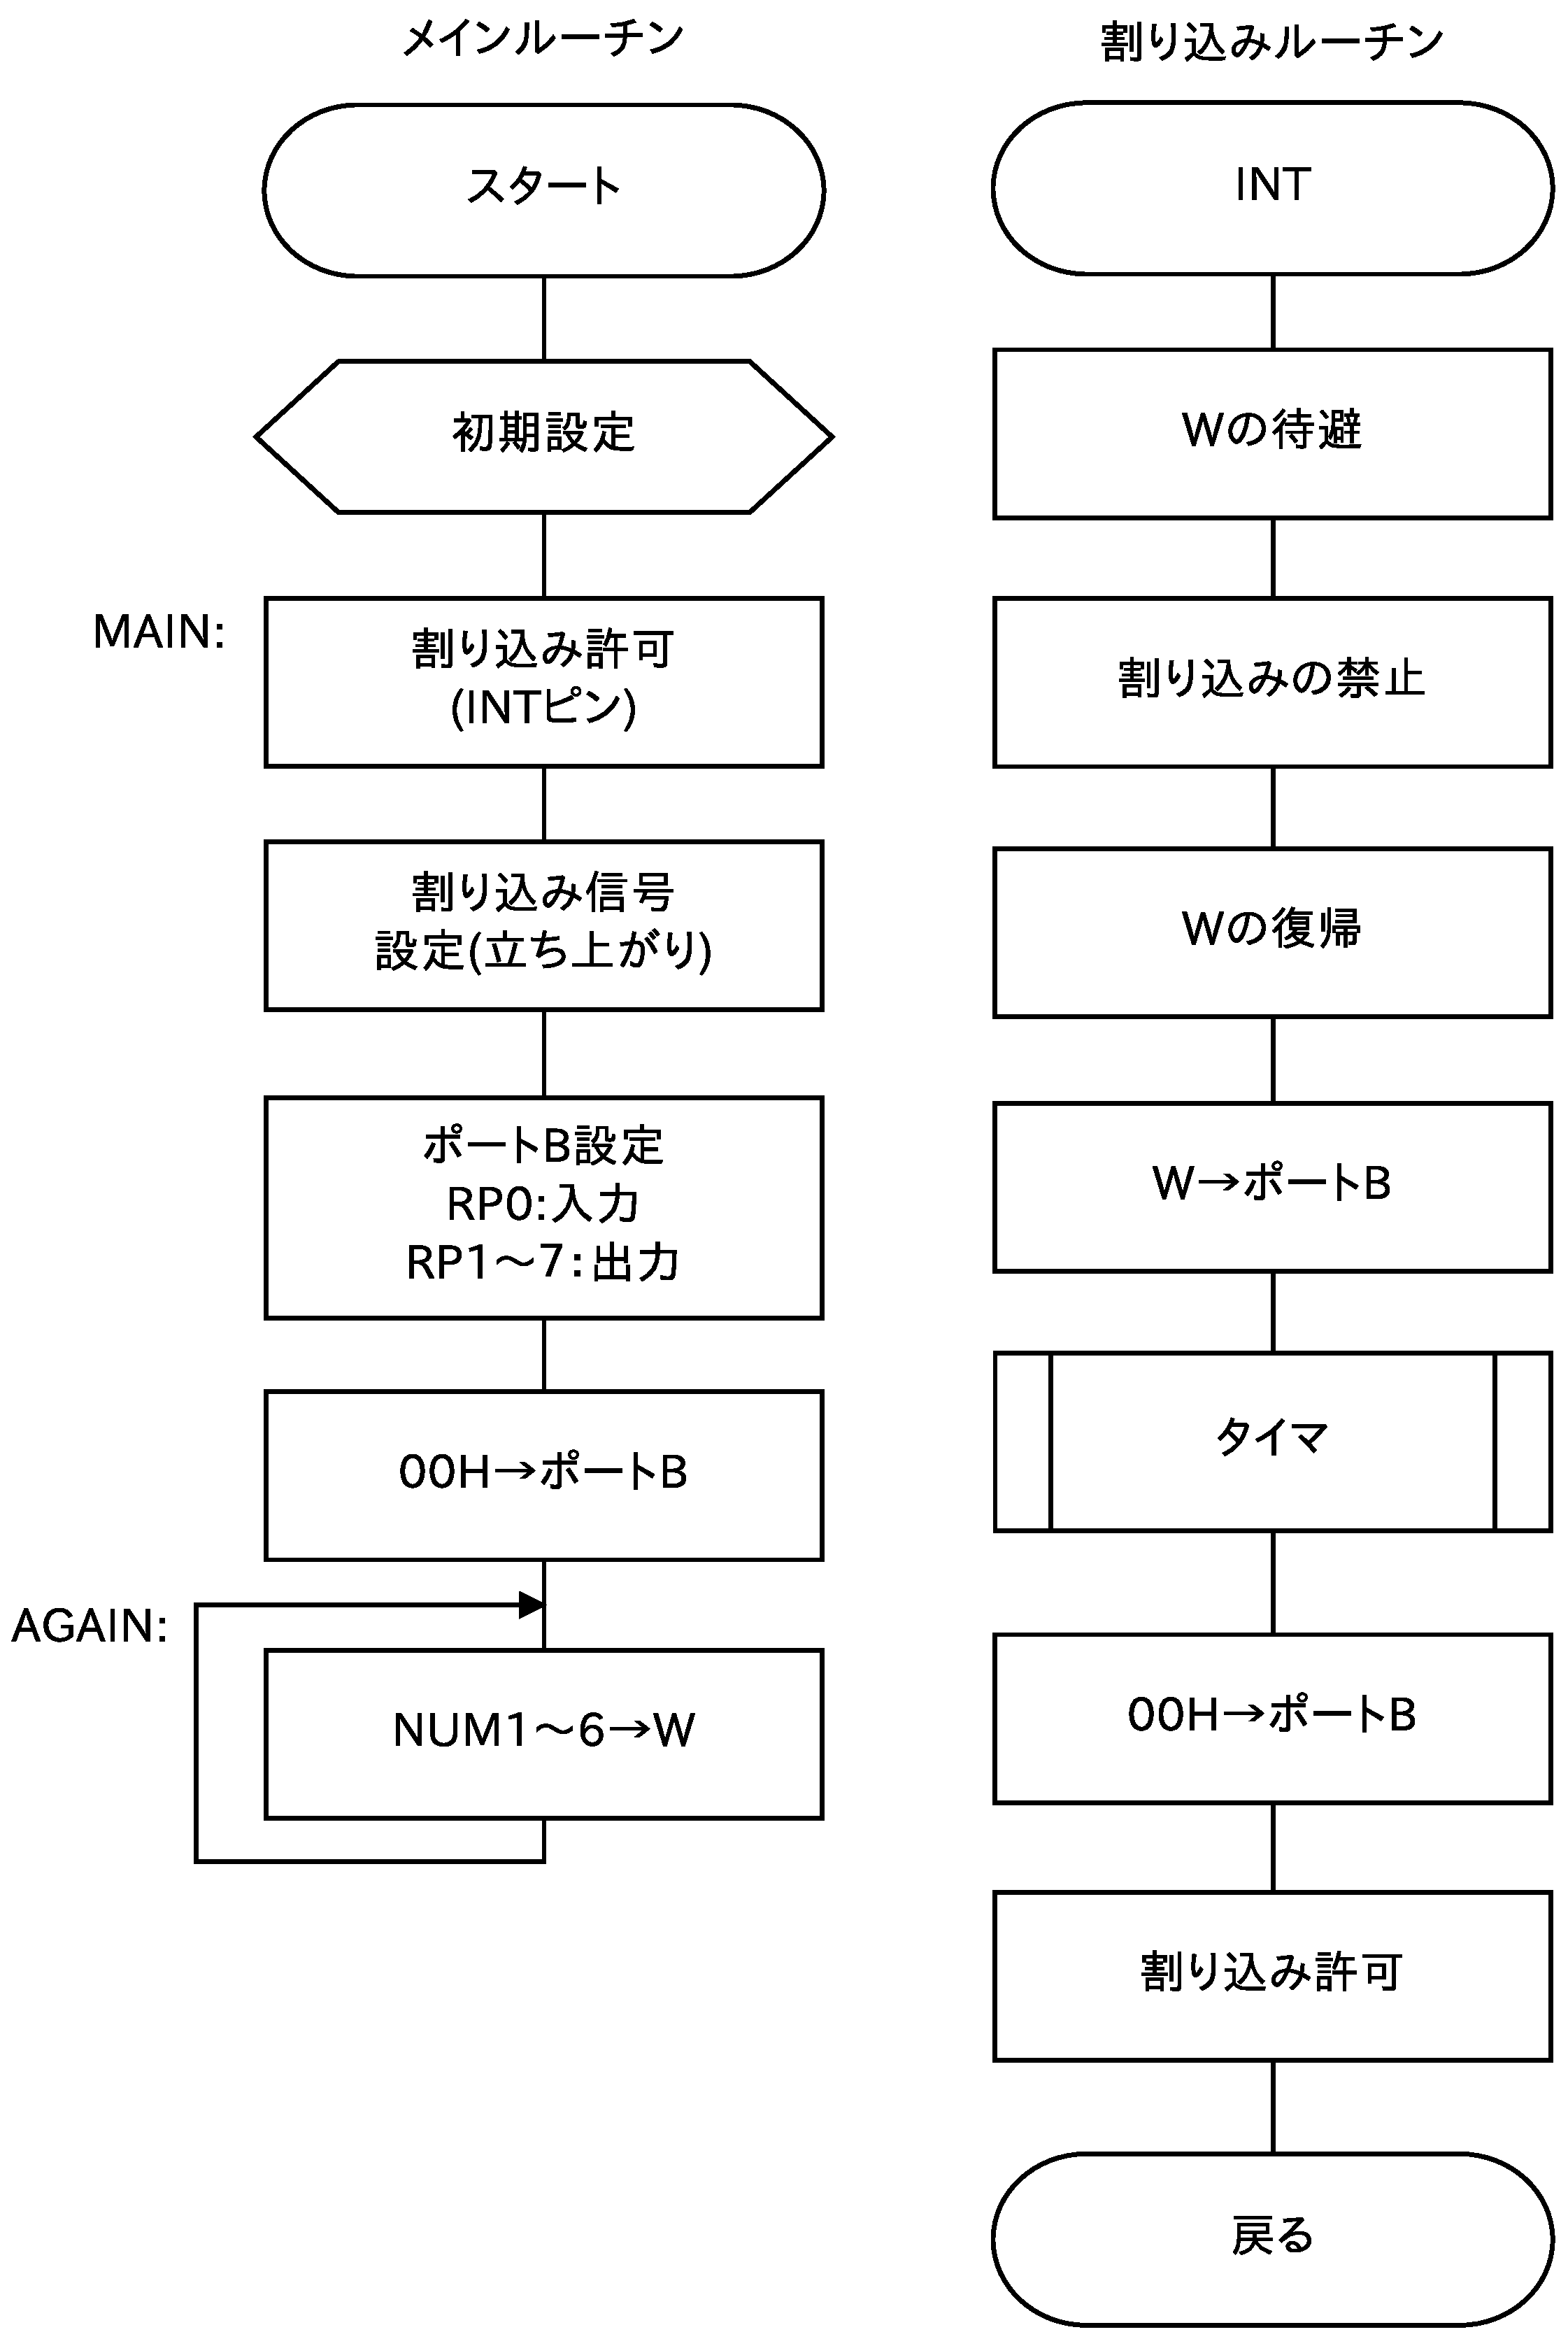
\includegraphics[height=200mm]{Diagram5-13.eps}
   \end{center}
   \caption{電子サイコロのプログラムのフローチャート}
   \label{fig:flow_5-13}
   \end{figure}
   \clearpage
  \subsection{実行結果・考察}
  プログラムを実行する前にボードのRB0をDOWNにしておく。
    \begin{figure}[htbp]
     \begin{center}
       \begin{tabular}{c|c|c}\hline
        目&76543210 & データ \\ \hline
         1&○○○●○○○○ & $10_{16}=00010000_2$ \\
         2&○○●○○○●○ & $22_{16}=00100010_2$\\
         3&○○●●○○●○ & $32_{16}=00110010_2$\\
         4&●○●○●○●○ & AA$_{16}=10101010_2$\\
         5&●○●●●○●○ & BA$_{16}=10111010_2$\\
         6&●●●○●●●○ & EE$_{16}=11101110_2$\\ \hline
       \end{tabular}\\
      ●:LED点灯 ○:LED消灯
      \caption{電子サイコロのプログラムの点灯パターン}
      \label{fig:out_5-13}
     \end{center}
    \end{figure}

    プログラムを実行するとLEDが消灯し、ボタン(RB0)を押すと図\ref{fig:out_5-13}のように目1〜6のいずれかのパターンのLEDが1秒間点灯し、その後全てのLED消灯する。
    LEDが点灯している時にボタン(RB0)を押しても反応しない。消灯したあとに再びボタン(RB0)を押すと目1〜6のいずれかのパターンのLEDが1秒間再び点灯する。この動作を繰り返した。\\

    INTCONレジスタは表\ref{INTCON}と表\ref{INTCON-bit}に示すような意味を持っている。
    INTCONレジスタを90$_{16}$にするということは\ref{INTCON}からGIEビットとINTEビットを
    1にすることでINT割り込み許可している。10$_{16}$についてはGIEビットを0にすることで全ての割り込みを禁止している。つまり00$_{16}$でも同じ意味を持つ。

    \begin{table}[htbp]
     \begin{center}
      \caption{INTCONレジスタの説明}
      \label{INTCON}
      \begin{tabular}{|c|c|c|c|c|c|c|c|c|c|}\hline
       \multirow{2}{*}{INTCON} &bit 7&bit 6&bit 5&bit 4&bit 3&bit 2&bit 1&bit 0& \\ \cline{2-9}
       &GIE&EEIE&TOIE&INTE&RBIE&TOIF&INTF&RBIF& \\ \hline
       許可のとき&1&0&0&1&0&0&0&0&90$_{16}$ \\
       禁止のとき&0&0&0&1&0&0&0&0&10$_{16}$ \\ \hline
      \end{tabular}
     \end{center}
    \end{table}

    \begin{table}[htbp]
     \begin{center}
      \caption{INTCONレジスタの各ビットの説明}
      \label{INTCON-bit}
      \begin{tabular}{|c|c|l|l|}\hline
       bit7&GIE&Global Interrupt Enable bit&全ての割り込み \\
       bit6&EEIE&EE Write Complete Interrupt Enable bit&EEPROM割り込み \\
       bit5&TOIE&TMR0 Overflow Interrupt Enable bit&タイマ0割り込み \\
       bit4&INTE&RB0/INT External Interrupt Enable bit&INT割り込み \\
       bit3&RBIE&RB Port Change Interrupt Enable bit&ポートB割り込み \\ \hline
       bit2&TOIF&TMR0 Overflow Interrupt Flag bit&タイマ0割り込み \\
       bit1&INTF&RB0/INT External Interrupt Flag bit&INT割り込み \\
       bit0&RBIF&RB Port Change Interrupt Flag bit&ポートB割り込み \\ \hline
      \end{tabular}

      bit7〜bit3は割り込み許可の時1に、禁止の時0にする。\\
      特にbit7が0なら全ての割り込みが禁止される。\\
      bit2〜bit0は割り込みが発生すると1がセットされる。\\
      再び割り込みを受け付けるには0にクリアしなければならない。\\
     \end{center}
    \end{table}

    NUM1は10$_{16}$という値で値そのものをWレジスタをポートBに転送することでLEDの点灯パターンにしている。
    一方、CNT1は0D$_{16}$というファイルレジスタを指していて、そのファイルレジスタの値をカウンタとして利用している。
    つまりNUM1は値を指していて、CNT1は値を保持する場所を指している。

    \begin{figure}[h]
      \begin{center}
       \begin{tabular}[t]{|ccc|}
        \hline
        \rule[0mm]{0mm}{7mm}③&   &⑤\\
        \rule[0mm]{0mm}{7mm}②& ④&⑥\\
        \rule[0mm]{0mm}{7mm}①&   &⑦\\ \hline
       \end{tabular}
   %全角スペースあり
       \begin{tabular}[t]{|ccc|}
        \hline
        \rule[0mm]{0mm}{7mm}●&   &●\\
        \rule[0mm]{0mm}{7mm}●& ●&●\\
        \rule[0mm]{0mm}{7mm}●&   &●\\ \hline
       \end{tabular}
   %全角スペースあり
       \begin{tabular}[t]{|ccc|}
        \hline
        \rule[0mm]{0mm}{7mm}●&   &○\\
        \rule[0mm]{0mm}{7mm}●& ●&●\\
        \rule[0mm]{0mm}{7mm}○
        &   &○\\ \hline
       \end{tabular}

     LED配置    'H'の点灯パターン 'L'の点灯パターン

       ●:LED点灯 ○:LED消灯
      \end{center}
       \caption{電子サイコロLED配置と'H','L'の点灯パターン}
       \label{fig-HL}
    \end{figure}

    'H'と'L'の点灯パターンを図\ref{fig-HL}のように設定するとする。すなわち、
    \begin{center}
       \begin{tabular}{c|c|c}\hline
        目&76543210 & データ \\ \hline
       'H'&●●●●●●●○ & FE$_{16}=11111110_2$ \\
       'L'&○●○●●●○○ & 5A$_{16}=01011100_2$\\ \hline
       \end{tabular}\\
      ●:LED点灯 ○:LED消灯
    \end{center}
      のように点灯データを設定する。したがって、プログラムのソースコードのうち、点灯パターンを設定している10〜15行目を以下のように変更する。
      \begin{lstlisting}[basicstyle=\ttfamily\footnotesize, frame=single]
10行目     NUM1    EQU     FEH     ;LEDの点灯データ'H'の設定
11行目     NUM2    EQU     5AH     ;LEDの点灯データ'L'の設定
12行目     NUM3    EQU     FEH     ;LEDの点灯データ'H'の設定
13行目     NUM4    EQU     5AH     ;LEDの点灯データ'L'の設定
14行目     NUM5    EQU     FEH     ;LEDの点灯データ'H'の設定
15行目     NUM6    EQU     5AH     ;LEDの点灯データ'L'の設定
      \end{lstlisting}
      これは単純にサイコロの目の6パターンを2パターンに置き替えた場合である。

      他の考え方として、点灯データは10行目と11行目だけで設定し、NUM3〜NUM6をWレジスタに書き込むところを減らすやり方がある。その場合は、10〜11行目と、65行目を次に変更し、12〜15行目と、53行目〜64行目を削除する。
      \begin{lstlisting}[basicstyle=\ttfamily\footnotesize, frame=single]
10行目     NUM1    EQU     FEH     ;LEDの点灯データ'H'の設定
11行目     NUM2    EQU     5AH     ;LEDの点灯データ'L'の設定
65行目             MOVLW   NUM2    ;
      \end{lstlisting}


 \clearpage
 \section{タイマ割り込み制御プログラム}
  \subsection{プログラムの説明}

2つの点灯パターンがタイマー割り込みで交互に繰り返すプログラム。繰り返しの周期を1秒にするため、タイマー割り込みの最大周期約26ms($\approx$4$\mu$s$\times 2^{16}=26.2144$ms)を38回繰り返してから点灯パターンが切り替わるようにしている。なお26.2144$\times$38=996.1472ms$\approx$1sである。

  メインルーチンでは、まず、RB0〜RB7をLEDの出力に設定する。タイマー割り込みを許可する。割り込み発生フラグをクリアし、割り込み回数カウンタCNTNを38回にして、データ設定フラグDATAFをクリアし、2番目の点灯データ(LEDD2)をPORTBに代入して、LEDを2番めの点灯パターンにする。次に、割り込み発生フラグをが1になるまで割り込み発生フラグの設定待ちループを繰り返す。割り込みが38回発生して、割り込み発生フラグがセットされていたら、次に進む。まず割り込み発生フラグをクリアする。もし、データ設定フラグDATAFがセットされていなかったら、点灯データを1番目(LEDD1)をPROTBに代入し、LEDを1番目の点灯パターンにする。データ設定フラグDATAFをセットする。そうではなくデータ設定フラグがセットされていたら、点灯データを2番目(LEDD2)をPROTBに代入し、LEDを2番目の点灯パターンにし、データ設定フラグをクリアする。 点灯パターンを変化させたあと、割り込み発生フラグの設定待ちのループを繰り返す。

  割り込みルーチンでは、タイマ割り込みが
約26ms毎に入るので割り込み回数カウンタを1減らす。もし、そのカウンタが0になれば割り込み発生フラグをセットする。すなわち26msを38回繰り返したあと(約1秒後)に割り込み発生フラグがセットされる。


  \subsection{フローチャート}
  図\ref{fig:flow_5-14}にこのプログラムのフローチャートを示す。
  \subsection{ソースコード}
  \begin{lstinputlisting}[basicstyle=\ttfamily\footnotesize, frame=single,numbers=left]
   {../5-14/5-14.asm}
  \end{lstinputlisting}
  \begin{figure}[htbp]
    \begin{center}
     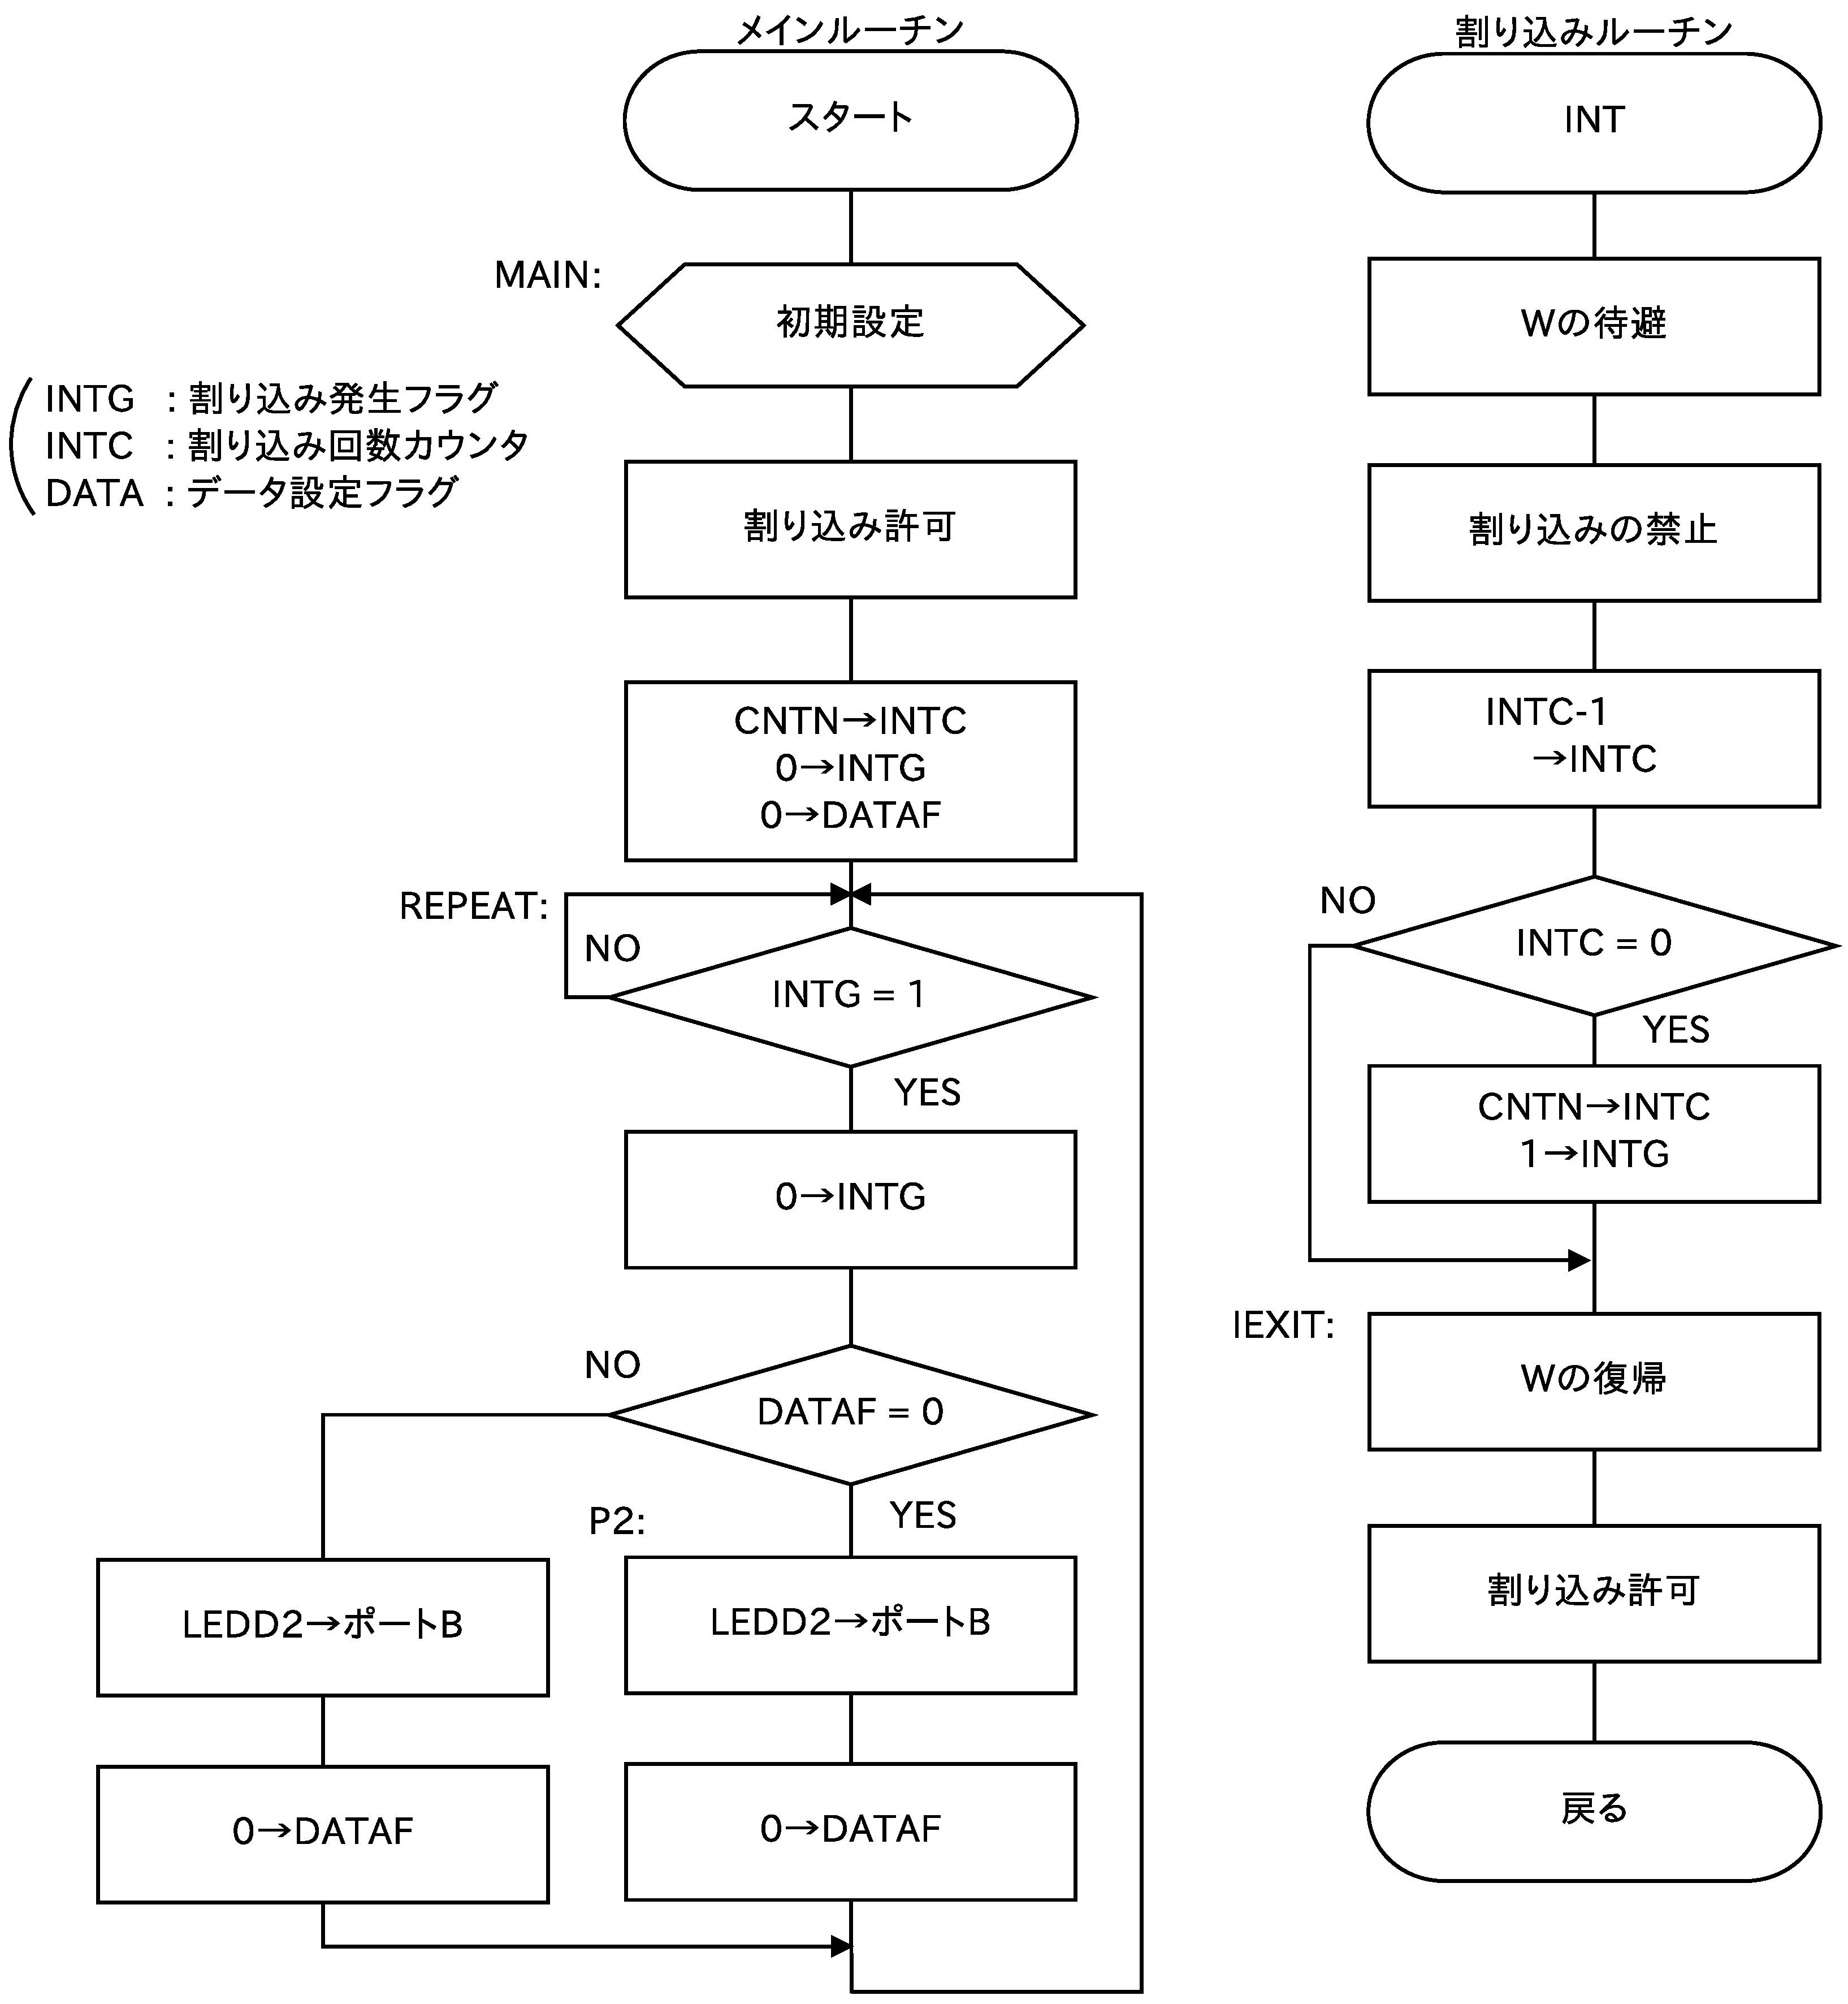
\includegraphics[height=200mm]{Diagram5-14.eps}
    \end{center}
   \caption{タイマ割り込み制御プログラムのフローチャート}
   \label{fig:flow_5-14}
  \end{figure}

  \clearpage
  \subsection{実行結果・考察}
  プログラムを実行する前にボードのRB0をDOWNにしておく。

  図\ref{fig:timer-int-led}に示す点灯パターンを1秒毎に繰り返した。プログラムスタート時はLEDD2の点灯パターンである。

  \begin{figure}
    \begin{center}
       \begin{tabular}{c|c|c}\hline
点灯パターン&76543210 & データ \\ \hline
      LEDD1 &●○●○●○●○ & 55$_{16}=11111110_2$ \\
      LEDD2 &○●○●○●○● & AA$_{16}=01011100_2$\\ \hline
       \end{tabular}\\
      ●:LED点灯 ○:LED消灯
    \end{center}
   \caption{タイマー割り込み制御プログラムのLED点灯パターン}
   \label{fig:timer-int-led}
  \end{figure}


  周期を500msに変更するにはタイマー割り込みのカウントを減らせば良い。今、38回カウントしているのを半分にすれば500msになる。ソースコードでは
      \begin{lstlisting}[basicstyle=\ttfamily\footnotesize, frame=single]
12行目     CNTN    EQU     D'19'   ;割り込み回数データ
      \end{lstlisting}
      を変更するだけでよい。この時の周期は$4\mu$s$\times 2^{16}\times 19=498.0736$msとなり、約0.5秒となる。

      点灯パターンを3種類にするには、データセットフラグDATAFを0,1の2種類ではなく3種類判定できるように変更すること、点灯パターンデータを3種類用意することである。
55行目から68行目を次に入れ替える。
      \begin{lstlisting}[basicstyle=\ttfamily\footnotesize, frame=single]
55行目 REPEAT  BTFSS   INTG,0          ;タイマ0割り込み発生フラグのチェック
56行目         GOTO    REPEAT          ;発生していなければ繰り返しチェック
57行目         BCF     INTG,0          ;発生していれば、フラグをクリア
58行目         BTFSC   DATAF,0         ;データ設定フラグ0ビット目は0か
59行目         GOTO    P2              ;1ならばパターン2へジャンプ
60行目         BTFSC   DATAF,1         ;データ設定フラグ1ビット目は0か
61行目         GOTO    P3              ;1ならばパターン3へジャンプ
62行目         MOVLW   LEDD2           ;0ならば点灯データ2をWレジスタにセット
63行目         MOVWF   PORTB           ;点灯データ2をポートBに出力
64行目         BSF     DATAF,0         ;データ設定フラグを01にセット
65行目         GOTO    REPEAT          ;繰り返し起点へジャンプ
66行目
67行目 P2      MOVLW   LEDD3           ;点灯データ3をWレジスタにセット
68行目         MOVWF   PORTB           ;点灯データ3をポートBに出力
69行目         BCF     DATAF,0         ;データ設定フラグを
70行目         BSF     DATAF,1         ;                 10にセット
71行目         GOTO    REPEAT          ;繰り返し起点へジャンプ
72行目
73行目 P3      MOVLW   LEDD1           ;点灯データ1をWレジスタにセット
74行目         MOVWF   PORTB           ;点灯データ1をポートBに出力
75行目         BCF     DATAF,0         ;データ設定フラグを
76行目         BCF     DATAF,1         ;                 00にセット
77行目         GOTO    REPEAT          ;繰り返し起点へジャンプ
      \end{lstlisting}

       データ設定フラグを2桁で考える。DATAF=00$_{16}$のときLEDD1のパターン、DATAF=01$_{16}$のときLEDD2のパターン、DATAF=02$_{16}$=011$_2$のときLEDD3の状態と考える。
       LEDD2$\to$LEDD3$\to$LEDD1$\to$LEDD2の順で変化するようにする。

       新たな点灯パターンの種類をLEDD3として、図\ref{fig:timer-LED3pattern}のように全点灯のパターンを追加する。
14行目と15行目の間に次を挿入。
      \begin{lstlisting}[basicstyle=\ttfamily\footnotesize, frame=single]
15行目LEDD3   EQU     0FFH            ;LED点灯データ3の設定
      \end{lstlisting}

   \begin{figure}
    \begin{center}
       \begin{tabular}{c|c|c}\hline
点灯パターン&76543210 & データ \\ \hline
      LEDD1 &●○●○●○●○ & 55$_{16}=11111110_2$ \\
      LEDD2 &○●○●○●○● & AA$_{16}=01011100_2$ \\
      LEDD3 &●●●●●●●● & FF$_{16}=111111111_2$\\ \hline
       \end{tabular}\\
      ●:LED点灯 ○:LED消灯
    \end{center}
    \caption{3種類の点灯パターン}
    \label{fig:timer-LED3pattern}
\end{figure}

変更したフローチャートを図\ref{fig:flow_5-14-1}に示す。
  \begin{figure}[htbp]
    \begin{center}
     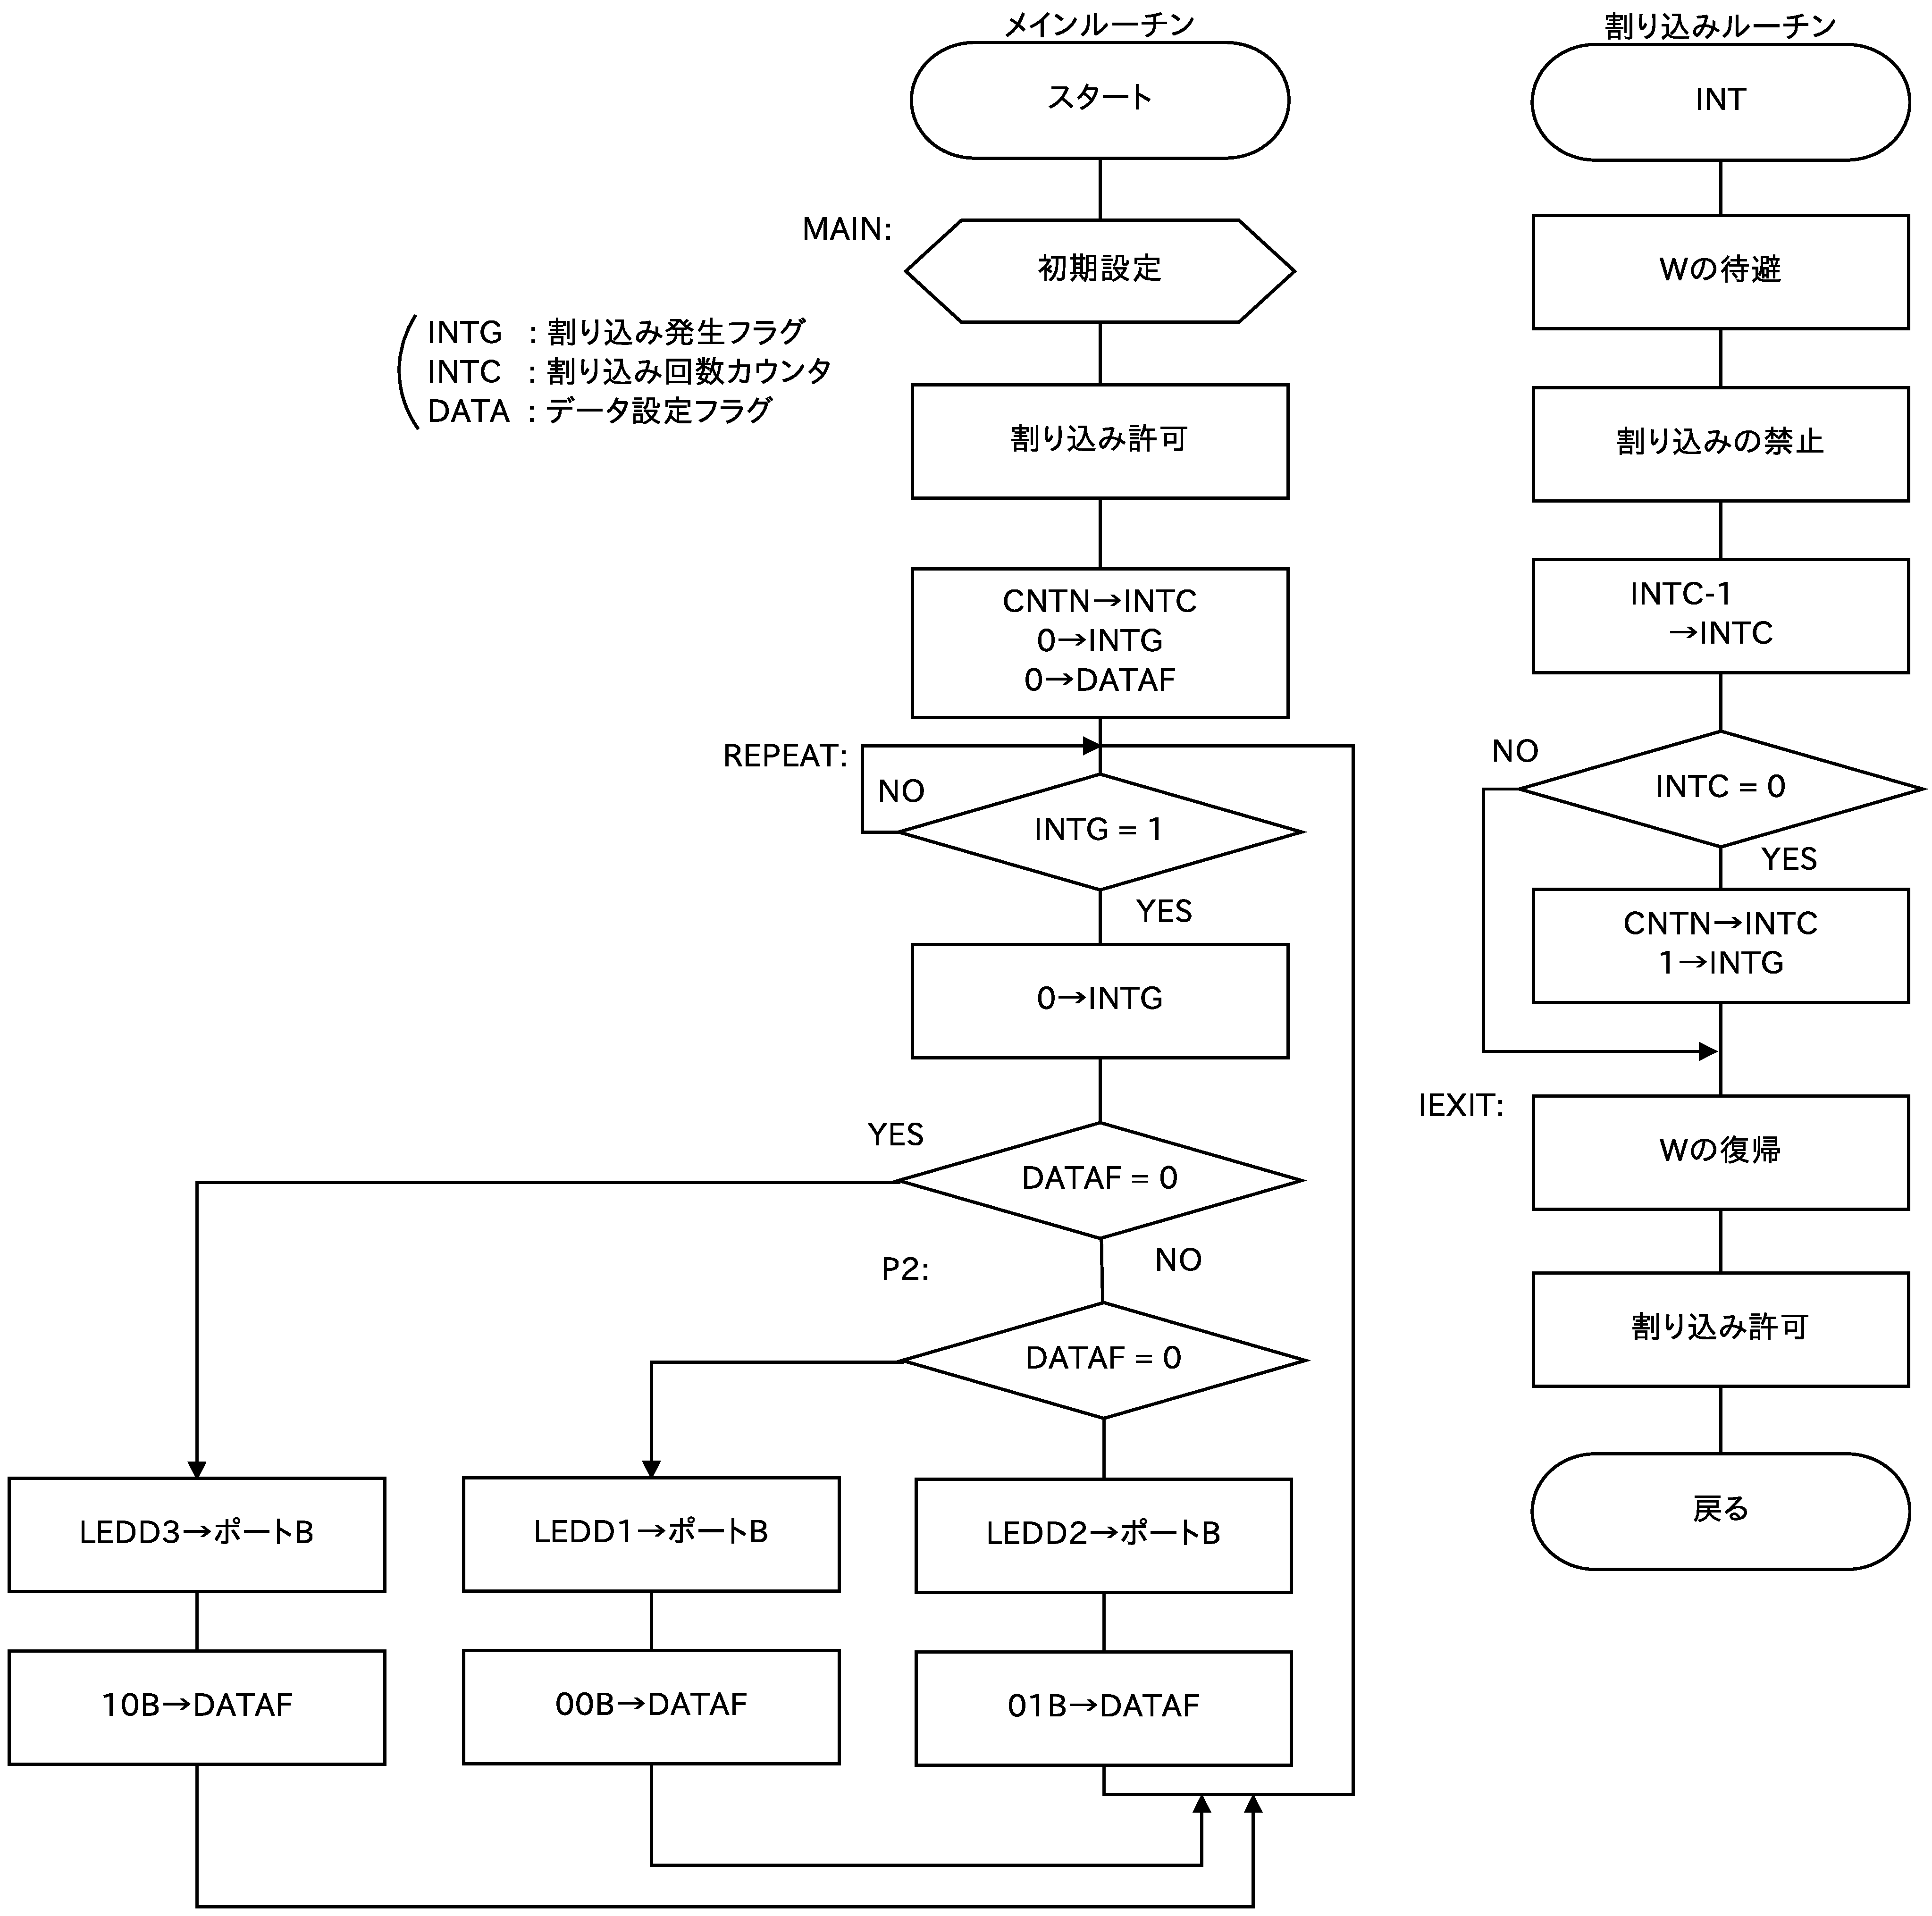
\includegraphics[height=180mm]{Diagram5-14-1.eps}
    \end{center}
   \caption{タイマ割り込み制御プログラムでLEDの点灯パターンが3種類の場合のフローチャート}
   \label{fig:flow_5-14-1}
  \end{figure}
\end{document}


